\documentclass[a0paper,portrait]{baposter}

\usepackage{wrapfig}
\usepackage{lmodern}
\usepackage{lipsum,graphicx}
\usepackage[utf8]{inputenc} %unicode support
\usepackage[T1]{fontenc}

\selectcolormodel{cmyk}

\graphicspath{{figures/}} % Directory in which figures are stored

\newcommand{\compresslist}{%
\setlength{\itemsep}{0pt}%
\setlength{\parskip}{1pt}%
\setlength{\parsep}{0pt}%
}

\newenvironment{boenumerate}
  {\begin{enumerate}\renewcommand\labelenumi{\textbf\theenumi.}}
  {\end{enumerate}}


\begin{document}

\definecolor{Mycolor1}{HTML}{00FFFF}
\definecolor{Mycolor2}{HTML}{008080}

\begin{poster}
{
grid=false,
headerborder=open, % Adds a border around the header of content boxes
colspacing=1em, % Column spacing
bgColorOne=white, % Background color for the gradient on the left side of the poster
bgColorTwo=white, % Background color for the gradient on the right side of the poster
borderColor=Mycolor1, % Border color
headerColorOne=Mycolor2, % Background color for the header in the content boxes (left side)
headerColorTwo=Mycolor2, % Background color for the header in the content boxes (right side)
headerFontColor=white, % Text color for the header text in the content boxes
boxColorOne=white, % Background color of the content boxes
textborder=rounded, %rectangle, % Format of the border around content boxes, can be: none, bars, coils, triangles, rectangle, rounded, roundedsmall, roundedright or faded
eyecatcher=false, % Set to false for ignoring the left logo in the title and move the title left
headerheight=0.11\textheight, % Height of the header
headershape=rounded, % Specify the rounded corner in the content box headers, can be: rectangle, small-rounded, roundedright, roundedleft or rounded
headershade=plain,
headerfont=\Large\textsf, % Large, bold and sans serif font in the headers of content boxes
%textfont={\setlength{\parindent}{1.5em}}, % Uncomment for paragraph indentation
linewidth=2pt % Width of the border lines around content boxes
}
{}
%
%----------------------------------------------------------------------------------------
%	TITLE AND AUTHOR NAME
%----------------------------------------------------------------------------------------
%
{

\vspace{1cm}
\textsf %Sans Serif
{
{\fontsize{18}{22}\selectfont \textcolor{red}{I}ntegrated \textcolor{red}{M}odelling of \textcolor{red}{PRO}TEIN Complexes \textcolor{red}{VI}A \textcolor{red}{S}ingle Shot Registration using \textcolor{red}{D}REAM (\textcolor{red}{IMPROVISeD})}
}
} % Poster title
% {\vspace{0.2em} Add Author Name, Add another author name\\ 
% {\small \vspace{0.7em} Department of Computing, TU Dublin, Tallaght, Dublin, Ireland}} 
{\sf\vspace{0.2em}\\
Ayush Raina, Rahul Chavan, Trishna Singh \\  
iGem Software Team, Indian Institute of Science, Banglore.\\


}
{
\includegraphics[width=.25\linewidth]{images/igem.png}} % TU Dublin logo


% this states the box starts at column 0 (edge of page), row 0 (top of page) for a span of 3 (columns wide)
\headerbox{1. Integrative Modelling Platform (IMP)}{name=introduction,column=0,row=0, span=2}{
\begin{enumerate}
    \item {\Large The IMP provides a computational approach designed to model the structure of macromolecular assemblies.}
    \item  {\Large It models large macromolecular complexes by integrating data from experiments, statistical analyses, physical principles, and prior models.}
\end{enumerate}

 %remove this, only added for spacing

}

\headerbox{2. Drawbacks of IMP}{name=drawbacks,column=2,row=0, span=1}{
    \begin{enumerate}
        \item {\Large Computationally expensive.} 
        \item {\Large Uses Markov Chain Monte Carlo (MCMC) sampling.}
    \end{enumerate}

    \vspace{0.45cm}
}

% this states the box starts at column 0 (edge of page), directly below the box labelled introduction for a span of 1 (column wide)
\headerbox{3. Proposed Method}{name=subtopic1,column=0,below=introduction,span=1}{

%\vspace{0.15cm}
\begin{enumerate}
    \item {\Large We propose to replace the MCMC sampling with a bottom-up approach.}
    \item {\Large We will use DREAM algorithm to replace the MCMC sampling.}
\end{enumerate}

\vspace{0.2cm} %remove this, only added for spacing

}



% this states the box starts at column 0 (edge of page), directly below the box labelled subtopic1 for a span of 1 (column wide)

\headerbox{4.1 Substrucutre Construction}{name=subtopic2,column=0,below=subtopic1,span=1}{
    {   
        \vspace{0.5cm}
        \hspace{0.5cm}
        \centering
    	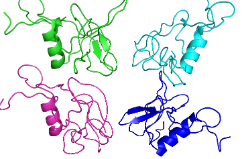
\includegraphics[scale=.7]{images/substructure.png}
    }

\vspace{0.9cm}
}

\headerbox{4.2 One-Shot Registration}{name=subtopic2,column=1,below=subtopic1,span=1}{
    \vspace{0.4cm}
    {   
        
        \hspace{0.7cm}
        \centering
    	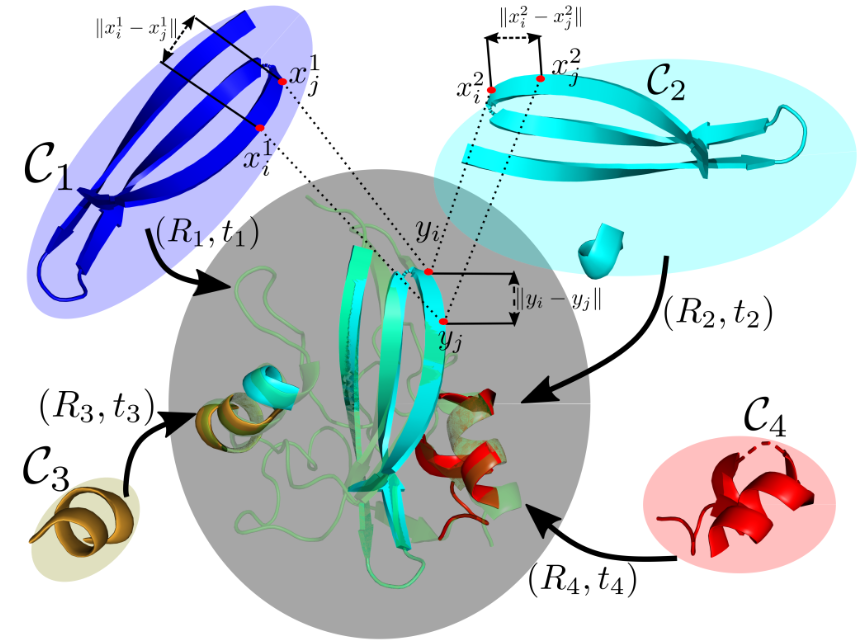
\includegraphics[scale=.2]{images/register.png}
    }

\vspace{0.4cm}

}

\headerbox{4.3 Gap Filling}{name=subtopic2gap,column=2,below=subtopic1,span=1}{
    {   
        \hspace{0.5cm}
        \centering
    	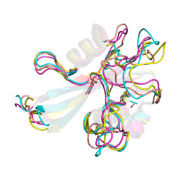
\includegraphics[scale=.8]{images/gap1.png}
    }


}

\headerbox{4. Distance Restraints and Energy Assisted Modelling (DREAM)}{name=subtopic3,column=1,below=introduction,span=2}{
{\Large This algorithm takes distance restraints data and models the structure of proteins which includes 3 steps:}


\begin{enumerate}
    \item {\Large Constructing the substrucutres.}
    \item {\Large One shot registration of all the substrucutres.}
    \item {\Large Gap filling using hybrid approached.}
\end{enumerate}

\vspace{0.01cm}
}


\headerbox{5. Graphical Overview of proposed method}{name=topicoverview,column=0,span=2,below=subtopic2}{

    {
        \hspace{1.5cm}
        \centering
    	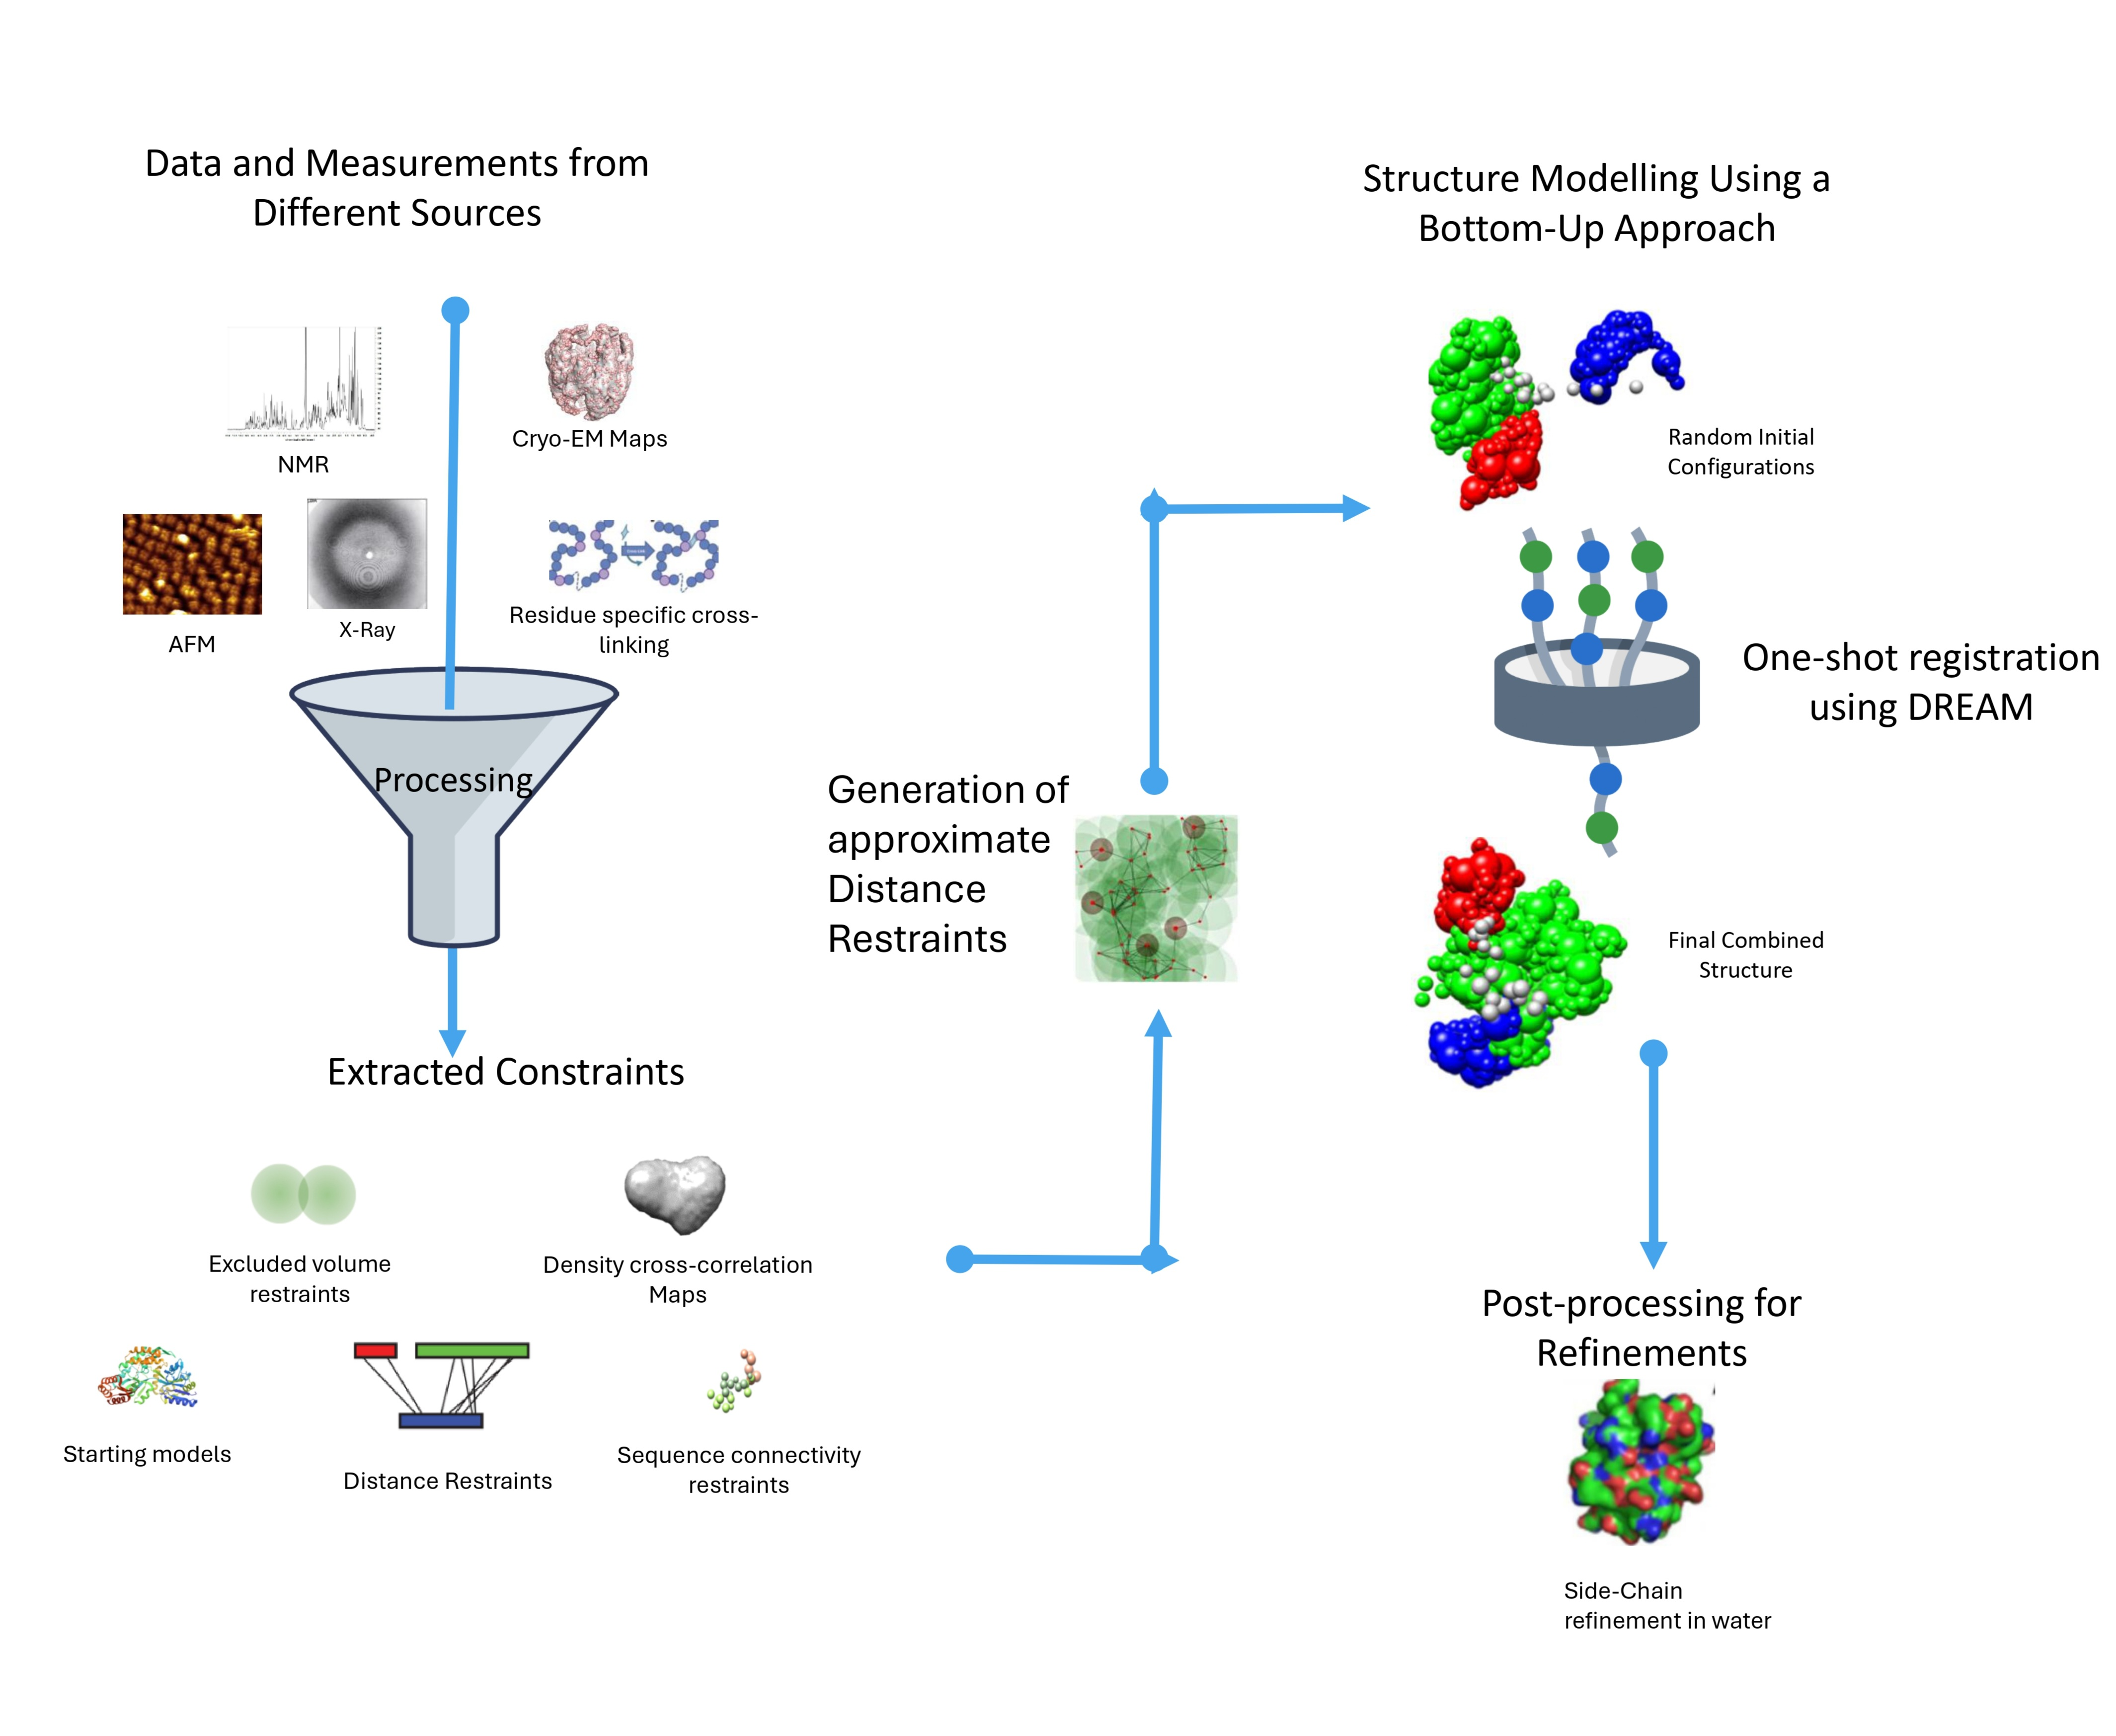
\includegraphics[scale=.08]{images/pipeline.jpeg}
    }
    \vspace{0.15cm}
}

\headerbox{8. Summary}{name=conclusion,column=0,below=topicoverview,span=2,above=bottom}{
\begin{enumerate}
    \item {\large Extract the distance restraints data from various experimental data.}
    \item {\large Use principle of DREAM algorithm to model the structure of complex.}
    \item {\large Generate the PDB file.}
\end{enumerate}

}

\headerbox{6. Human Practices}{name=hp,column=2,below=subtopic2gap,span=1}{
\subsubsection*{3R's}
\begin{enumerate}
    \item {\large Replacement}
    \item {\large Reduction}
    \item {\large Refinement}
\end{enumerate}

\subsection*{Our Stakeholders}
\begin{enumerate}
    \item {\large Professors}
    \item {\large Research Students}
    \item {\large Protein Modelling Companies}
\end{enumerate}
\vspace{0.05cm}
}

\headerbox{7. Our Mentors}{name=mentors,column=2,below=hp,span=1}{
    \begin{enumerate}
        \item {\Large Professor Debnath Pal (CDS IISc)}
        \item {\Large Dr. Shruthi (NCBS)}
    \end{enumerate}
    
    \vspace{0.45cm}
}

\headerbox{9. Links and Resources}{name=last,column=2,below=mentors,span=1,above=bottom} {
    {   
        
        \hspace{2.6cm}
        \centering
    	
\includegraphics[scale=.015]{images/qr.png}
    }
}

\end{poster}

\end{document}
